\documentclass[11pt]{article}

\usepackage[T1]{fontenc}
\usepackage[utf8]{inputenc}
\usepackage[a4paper,margin=1in]{geometry}
\usepackage{amsmath,amssymb,amsthm,mathtools}
\usepackage{bm}
\usepackage{graphicx}
\usepackage{subcaption}
\usepackage{booktabs}
\usepackage[colorlinks=true,linkcolor=blue,citecolor=blue,urlcolor=blue]{hyperref}

\graphicspath{{Rapport/}{./}}

\newtheorem{theorem}{Th\'eor\`eme}[section]
\newtheorem{lemma}[theorem]{Lemme}
\newtheorem{proposition}[theorem]{Proposition}
\newtheorem{corollary}[theorem]{Corollaire}
\theoremstyle{remark}
\newtheorem{remark}[theorem]{Remarque}
\theoremstyle{definition}
\newtheorem{definition}[theorem]{D\'efinition}

\title{TP Kalman}

\author{
  Fatimetou Narjah \and Mohamed Benloughmari
}
\date{}

\begin{document}

\maketitle

\section{Mod\`ele et notations}\label{sec:modele}

\subsection{Mod\`ele d'\'evolution}

L'\'etat est $x = [p\ v]^\top$ avec $p = [p_x\ p_y\ p_z]^\top$ la position et
$v = [v_x\ v_y\ v_z]^\top$ la vitesse. Le mod\`ele d'\'evolution est lin\'eaire, sans commande, \`a
vitesse quasi constante :

\begin{equation}
x_{k+1} = F\, x_k + w_k,
\qquad
w_k \sim \mathcal{N}(0, Q),
\label{eq:evolution}
\end{equation}

avec $\Delta T = 1$ et

\begin{equation}
F =
\begin{bmatrix}
I_3 & I_3 \\[2pt]
0_3 & I_3
\end{bmatrix},
\qquad
Q =
\begin{bmatrix}
q_p I_3 & 0_3 \\[2pt]
0_3 & q_v I_3
\end{bmatrix},
\quad q_p = 10^{-4},\ q_v = 10^{-2}.
\label{eq:FQ}
\end{equation}

\subsection{Mod\`ele d'observation}

On observe les trois coordonn\'ees de position :

\begin{equation}
y_k = H\, x_k + v_k,
\qquad
v_k \sim \mathcal{N}(0, R),
\qquad
H = \begin{bmatrix} I_3 & 0_{3\times 3} \end{bmatrix},
\qquad
R = 100\, I_3 .
\label{eq:obs}
\end{equation}

L'\'ecart-type de mesure vaut donc $\sigma = 10\ \text{m}$. L'initialisation est
$x_0 = 0_6$ et $P_0 = \operatorname{diag}(10^4, 10^4, 10^4, 10^2, 10^2, 10)$.

\section{Filtre de Kalman lin\'eaire}\label{sec:kalman}

On rappelle les \'equations du filtre. \'Etant donn\'es $\hat{x}_{k|k}$ et $P_{k|k}$ :

\begin{align}
\text{Pr\'ediction :}&&
\hat{x}_{k+1|k} &= F\, \hat{x}_{k|k}, &
P_{k+1|k} &= F\, P_{k|k}\, F^\top + Q, \label{eq:predict} \\
\text{Innovation :}&&
\nu_{k+1} &= y_{k+1} - H\, \hat{x}_{k+1|k}, &
S_{k+1} &= H\, P_{k+1|k}\, H^\top + R, \label{eq:innov} \\
\text{Gain :}&&
K_{k+1} &= P_{k+1|k}\, H^\top\, S_{k+1}^{-1}, \label{eq:gain} \\
\text{Correction :}&&
\hat{x}_{k+1|k+1} &= \hat{x}_{k+1|k} + K_{k+1}\,\nu_{k+1}, &
P_{k+1|k+1} &= \bigl(I - K_{k+1} H\bigr)\, P_{k+1|k}. \label{eq:corr}
\end{align}

\section{Croissance de la covariance pendant un trou de mesure}\label{sec:trou}

On s'int\'eresse au comportement de la covariance lorsque les observations sont indisponibles,
c'est-\`a-dire lorsque seule l'\'etape de pr\'ediction \eqref{eq:predict} est ex\'ecut\'ee.
Num\'eriquement, on observe sur les bandes $\pm 3\sigma$ que la variance de position cro\^it alors que
la variance de vitesse reste quasi constante. Nous le prouvons par calcul exact, avec la matrice $F$
compl\`ete.

\subsection{R\'ecurrences par blocs}

On partitionne la covariance en blocs $3\times 3$ :

\begin{equation}
P_k =
\begin{bmatrix}
P_{pp,k} & P_{pv,k} \\[2pt]
P_{vp,k} & P_{vv,k}
\end{bmatrix},
\end{equation}

o\`u $P_{pp,k}$ est la variance de position, $P_{vv,k}$ celle de vitesse, et
$P_{pv,k} = P_{vp,k}^\top$ la covariance crois\'ee position--vitesse.

\begin{lemma}\label{lem:blocs}
Pendant le trou de mesure, la covariance suit les r\'ecurrences par blocs
\begin{equation}
\boxed{\begin{aligned}
P_{pp,k+1} &= P_{pp,k} + P_{pv,k} + P_{vp,k} + P_{vv,k} + q_p\, I_3, \\[2pt]
P_{pv,k+1} &= P_{pv,k} + P_{vv,k}, \\[2pt]
P_{vp,k+1} &= P_{vp,k} + P_{vv,k}, \\[2pt]
P_{vv,k+1} &= P_{vv,k} + q_v\, I_3.
\end{aligned}}
\label{eq:blocs}
\end{equation}
\end{lemma}

\begin{proof}
Sans observation, la covariance suit \eqref{eq:predict} avec $P_{k+1} = F P_k F^\top + Q$. Le produit
$F P_k F^\top$ s'\'ecrit

\begin{equation}
F P_k F^\top =
\begin{bmatrix}
P_{pp,k} + P_{pv,k} + P_{vp,k} + P_{vv,k} & P_{pv,k} + P_{vv,k} \\[2pt]
P_{vp,k} + P_{vv,k} & P_{vv,k}
\end{bmatrix},
\end{equation}

et l'ajout de $Q = \operatorname{diag}(q_p I_3, q_v I_3)$ donne imm\'ediatement \eqref{eq:blocs}.
\end{proof}

\subsection{D\'ecouplage par axe}

Les matrices $F$, $Q$, $H$ et $R$ \'etant diagonales par blocs (un bloc $2\times 2$ par axe), tous les
blocs $P_{pp}$, $P_{pv}$, $P_{vp}$, $P_{vv}$ sont eux-m\^emes diagonaux. Chaque axe $(x,y,z)$ suit donc
une r\'ecurrence scalaire ind\'ependante. Pour un axe donn\'e, on pose

\begin{equation}
a_k = (P_{pp,k})_{ii},
\qquad
b_k = (P_{pv,k})_{ii} = (P_{vp,k})_{ii},
\qquad
c_k = (P_{vv,k})_{ii},
\end{equation}

et les r\'ecurrences \eqref{eq:blocs} se r\'eduisent \`a

\begin{equation}
\boxed{\begin{aligned}
a_{k+1} &= a_k + 2b_k + c_k + q_p, \\[2pt]
b_{k+1} &= b_k + c_k, \\[2pt]
c_{k+1} &= c_k + q_v.
\end{aligned}}
\label{eq:scalaires}
\end{equation}

\subsection{Variance de vitesse : croissance lin\'eaire}

\begin{proposition}\label{prop:vitesse}
La variance de vitesse cro\^it lin\'eairement : $c_k = c_0 + k\, q_v$.
\end{proposition}

\begin{proof}
La troisi\`eme r\'ecurrence de \eqref{eq:scalaires} donne imm\'ediatement $c_k = c_0 + k\, q_v$.
La pente $q_v = 10^{-2}$ est tr\`es faible : sur 10 pas, $c_{10} - c_0 = 0.1$, \`a comparer \`a
$c_0 \approx 0.14$ en r\'egime stationnaire. L'\'ecart-type
$\sigma_v(k) = \sqrt{c_0 + k\, q_v}$ varie donc peu, ce qui explique que la bande $\pm 3\sigma_v$
\emph{semble constante}.
\end{proof}

\subsection{Variance de position : croissance quadratique}

\begin{proposition}\label{prop:position}
La variance de position admet la forme ferm\'ee
\begin{equation}
\boxed{a_k = a_0 + (2b_0 + c_0 + q_p)\, k + c_0\, k\,(k-1) + q_v\,\frac{k\,(k-1)\,(2k-1)}{6}}
\label{eq:position}
\end{equation}
et cro\^it quadratiquement au premier ordre, $a_k \sim c_0\, k^2$.
\end{proposition}

\begin{proof}
De $b_{k+1} = b_k + c_k$ on d\'eduit
\begin{equation}
b_k = b_0 + k\, c_0 + q_v\,\frac{k\,(k-1)}{2}.
\end{equation}
En injectant dans la r\'ecurrence de $a$ puis en sommant, on obtient \eqref{eq:position}. Le terme
dominant est quadratique : $a_k \sim c_0\, k^2$, le terme cubique en $q_v$ \'etant n\'egligeable devant
lui. En effet la d\'eriv\'ee seconde discr\`ete vaut
\begin{equation}
\Delta^2 a_k \coloneqq \Delta a_{k+1} - \Delta a_k = 2 c_k + q_v = 2 c_0 + q_v + 2 q_v k \approx 2 c_0,
\end{equation}
constante au premier ordre, signature d'une croissance quadratique. L'\'ecart-type, lui, cro\^it
lin\'eairement : $\sigma_p(k) = \sqrt{a_k} \sim \sqrt{c_0}\ k$.
\end{proof}

\begin{remark}
C'est donc bien l'\'ecart-type $\sigma$ (ce qui est trac\'e) qui est lin\'eaire pour la position et
quasi constant pour la vitesse. En termes de variance : la position cro\^it \emph{quadratiquement}
(terme dominant $c_0 k^2$), tandis que la vitesse cro\^it \emph{lin\'eairement}, avec une pente $q_v$
si faible qu'elle para\^it constante.
\end{remark}

\subsection{Interpr\'etation}

La vitesse ne subit qu'une d\'erive additive constante : \`a chaque pas, le filtre ajoute un doute fixe
$q_v$, qui ne se r\'epercute pas sur lui-m\^eme. La position, elle, int\`egre la vitesse
($p_{k+1} = p_k + v_k$) : chaque pas ajoute l'incertitude de vitesse accumul\'ee, d'o\`u une croissance
acc\'el\'er\'ee. C'est le comportement typique de la navigation \`a l'estime sans recalage externe.

\section{Filtre de Kalman \'etendu : croissance de la variance de vitesse}\label{sec:ekf}

On consid\`ere le mod\`ele de la question Q0b : un objet se d\'eplace sur un axe, d'\'etat
$[s\ v]^\top$ (position, vitesse), et un capteur plac\'e en $(x_s, y_s) = (0, -20)$ mesure un
angle bruit\'e $z = h(s) + \text{bruit}$, avec

\begin{equation}
h(s) = \operatorname{atan2}(-y_s,\ s - x_s) = \operatorname{atan2}(20,\ s).
\label{eq:h-bearing}
\end{equation}

La jacobienne d'observation vaut $H = \begin{bmatrix} h_s & 0 \end{bmatrix}$, avec

\begin{equation}
h_s = \frac{y_s}{(s-x_s)^2 + y_s^2} = \frac{-20}{s^2 + 400},
\label{eq:hs}
\end{equation}

et les bruits sont $q_p = 10^{-4}$, $q_v = 10^{-2}$ (dynamique) et
$R = (1^\circ\ \text{en radians})^2 \approx 3.05\times 10^{-4}$ (mesure).

On note la covariance $P = \begin{bmatrix} a & b \\ b & c \end{bmatrix}$, avec
$a = \operatorname{var}(s)$, $c = \operatorname{var}(v)$ (variance de vitesse) et
$b = \operatorname{cov}(s,v)$.

\textbf{Pr\'ediction} ($F P F^\top + Q$, avec $q_p = 10^{-4}$, $q_v = 10^{-2}$) :

\begin{equation}
a_{\text{pred}} = a + 2b + c + q_p,
\qquad
b_{\text{pred}} = b + c,
\qquad
c_{\text{pred}} = c + q_v .
\end{equation}

\textbf{Correction} avec $H = \begin{bmatrix} h_s & 0 \end{bmatrix}$ :

\begin{equation}
S = h_s^2\, a_{\text{pred}} + R,
\qquad
K = P_{\text{pred}} H^\top S^{-1}
= \frac{1}{S}\begin{bmatrix} h_s\,a_{\text{pred}} \\ h_s\,b_{\text{pred}} \end{bmatrix}.
\end{equation}

Le bloc $(2,2)$ de $P_{\text{corr}} = (I - KH) P_{\text{pred}}$ donne la nouvelle variance de
vitesse :

\begin{equation}
c_{\text{corr}} = c_{\text{pred}} - \frac{h_s^2\, b_{\text{pred}}^2}{S}
= c_{\text{pred}} - \frac{h_s^2\, b_{\text{pred}}^2}{h_s^2\, a_{\text{pred}} + R}.
\end{equation}

D'o\`u la r\'ecurrence compl\`ete :

\begin{equation}
\boxed{\,c_{k+1} = c_k + q_v - \frac{h_s^2\,(b_k + c_k)^2}{\,h_s^2\,(a_k + 2b_k + c_k + q_p) + R\,}\,}
\label{eq:ekf-recurrence}
\end{equation}

\textbf{Lecture de la formule}

\begin{enumerate}
\item \textbf{Terme $+q_v$} : \`a chaque pr\'ediction, le bruit de dynamique injecte
  $q_v = 10^{-2}$ d'incertitude sur la vitesse. C'est le moteur de la croissance.

\item \textbf{Terme de correction $-\dfrac{h_s^2 b_{\text{pred}}^2}{S}$} : c'est la seule chose
  qui tire la variance de vitesse vers le bas. Or la mesure d'angle n'observe pas directement la
  vitesse ($H$ a une composante nulle sur $v$) : la vitesse n'est corrig\'ee qu'indirectement,
  via sa covariance crois\'ee $b$ avec la position.

\item \textbf{R\^ole de $h_s \to 0$} : quand l'objet s'\'eloigne, $h_s = -20/(s^2+400) \to 0$.
  Alors le num\'erateur $h_s^2 b_{\text{pred}}^2 \to 0$ (et $S \to R$, non nul), donc le terme de
  correction s'annule. La r\'ecurrence se r\'eduit \`a
  \begin{equation}
  c_{k+1} \approx c_k + q_v .
  \end{equation}
  La variance de vitesse cro\^it alors lin\'eairement, avec une pente $q_v = 10^{-2}$.
\end{enumerate}

\section{Influence des bruits $Q$ et $R$}\label{sec:bruits}

Le bruit de dynamique $Q$ quantifie la confiance du filtre dans son mod\`ele de mouvement. Lorsque $Q$
augmente, $P_{k+1|k} = F P F^\top + Q$ est plus grand, donc le gain $K$ est plus grand : le filtre
accorde plus de poids aux mesures, l'estimation devient r\'eactive mais plus bruit\'ee. \`A l'inverse,
un $Q$ faible rend le filtre confiant dans son mod\`ele, l'estimation plus lisse mais plus lente \`a
r\'eagir.

Le bruit de mesure $R$ quantifie la confiance du filtre dans ses capteurs. Lorsque $R$ augmente,
$S = H P H^\top + R$ est plus grand, donc $K$ est plus petit : les mesures sont jug\'ees peu fiables,
l'estimation est liss\'ee mais moins pr\'ecise. \`A l'inverse, un $R$ faible rend les mesures quasi
parfaites et l'estimation colle aux observations, en amplifiant leur bruit.

\begin{figure}[htbp]
    \centering
    \begin{subfigure}[b]{0.48\textwidth}
        \centering
        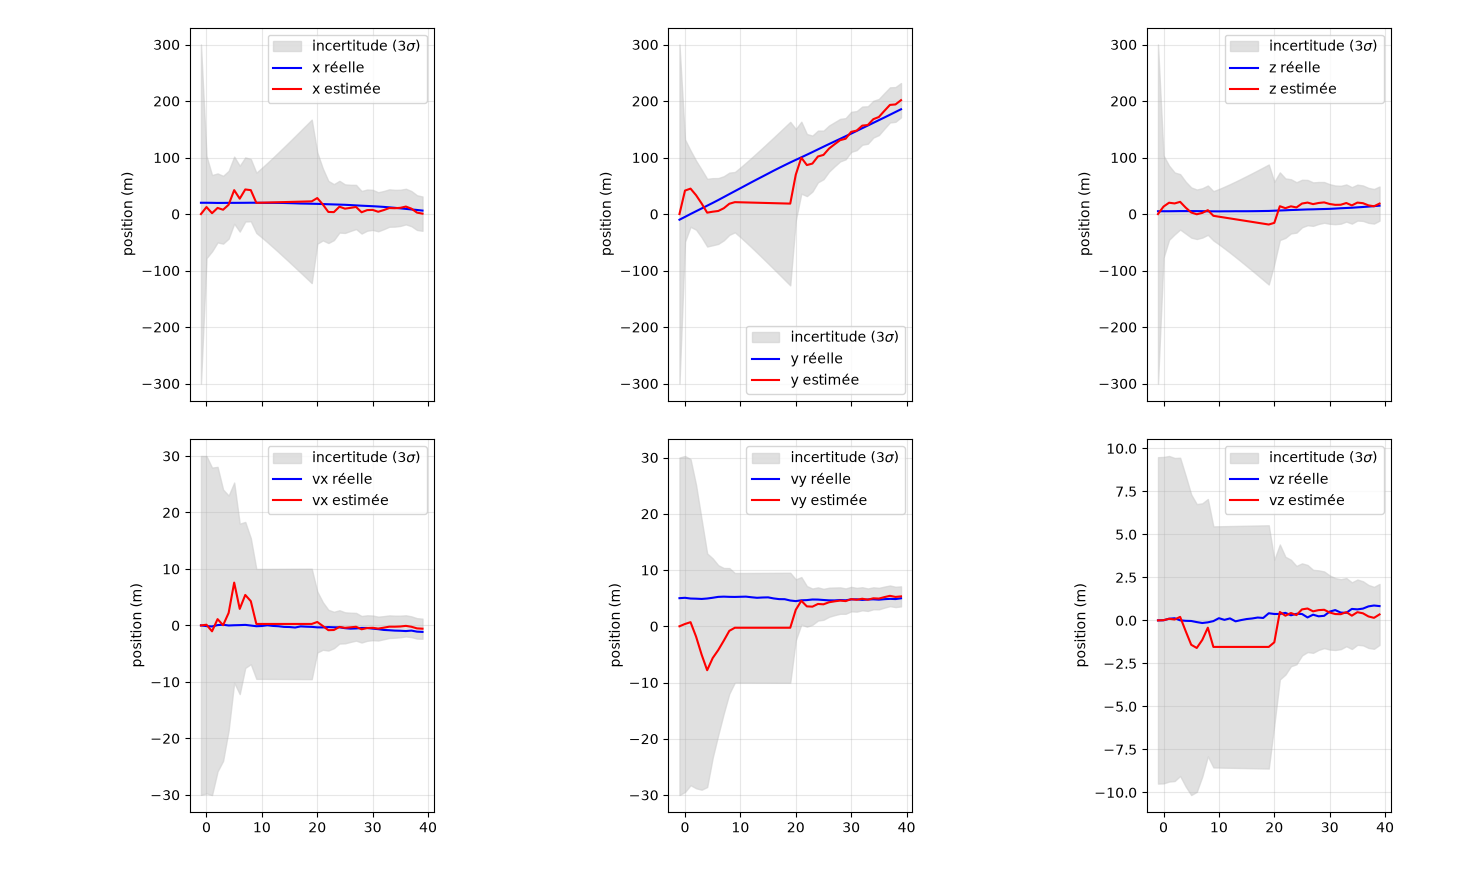
\includegraphics[width=\textwidth]{10Rk.png}
        \caption{Variation de $R$.}
        \label{fig:R}
    \end{subfigure}
    \hfill
    \begin{subfigure}[b]{0.48\textwidth}
        \centering
        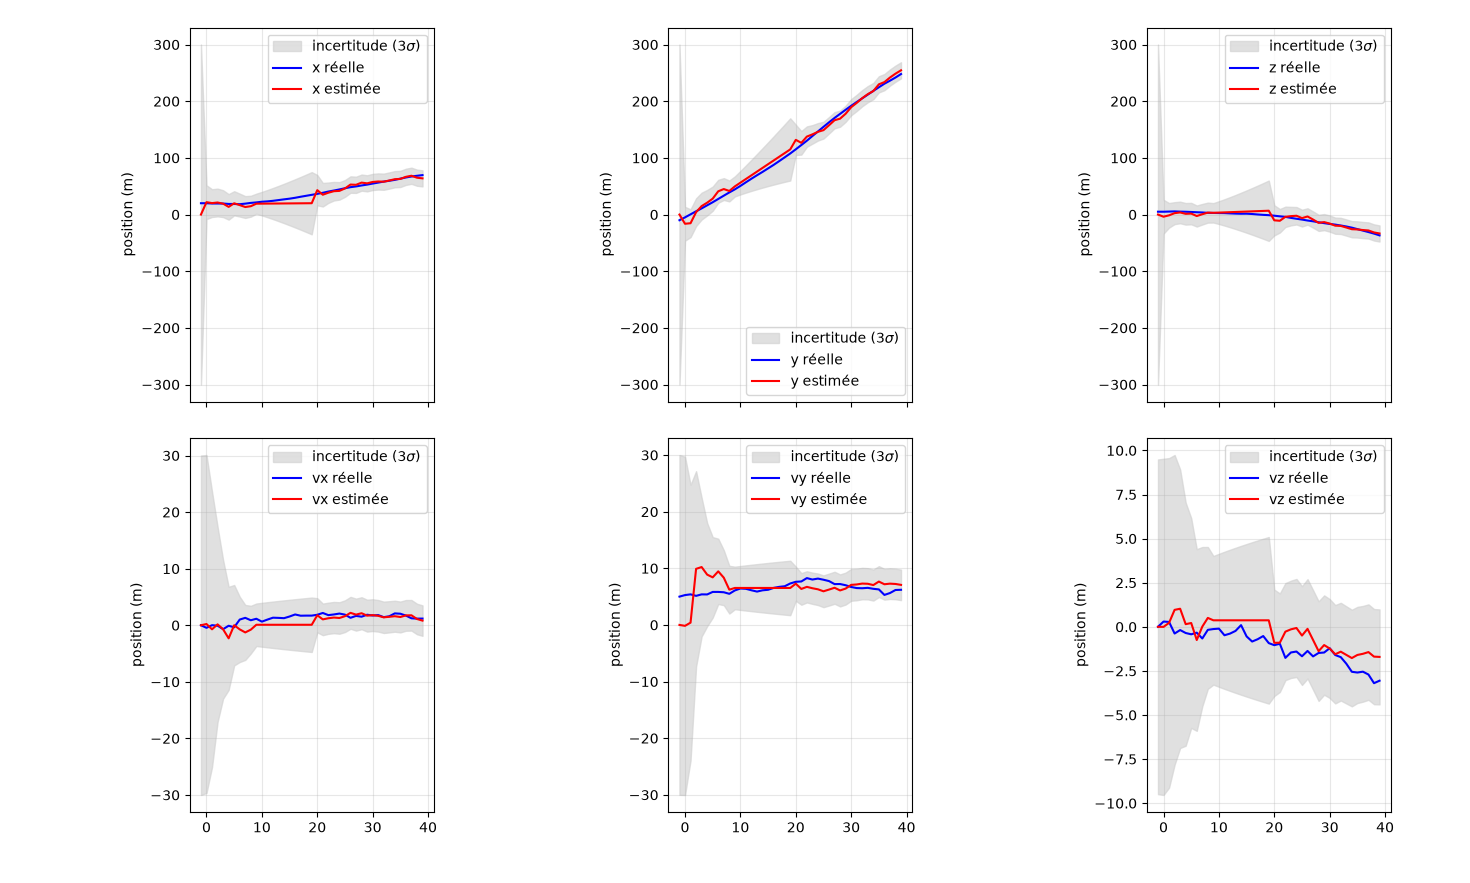
\includegraphics[width=\textwidth]{20Qk.png}
        \caption{Variation de $Q$.}
        \label{fig:Q}
    \end{subfigure}
    \caption{Influence des bruits de mesure $R$ et de dynamique $Q$ sur l'estimation
    (position r\'eelle en bleu, estim\'ee en rouge, bande $\pm 3\sigma$ en gris).}
    \label{fig:bruits}
\end{figure}

\begin{figure}[htbp]
    \centering
    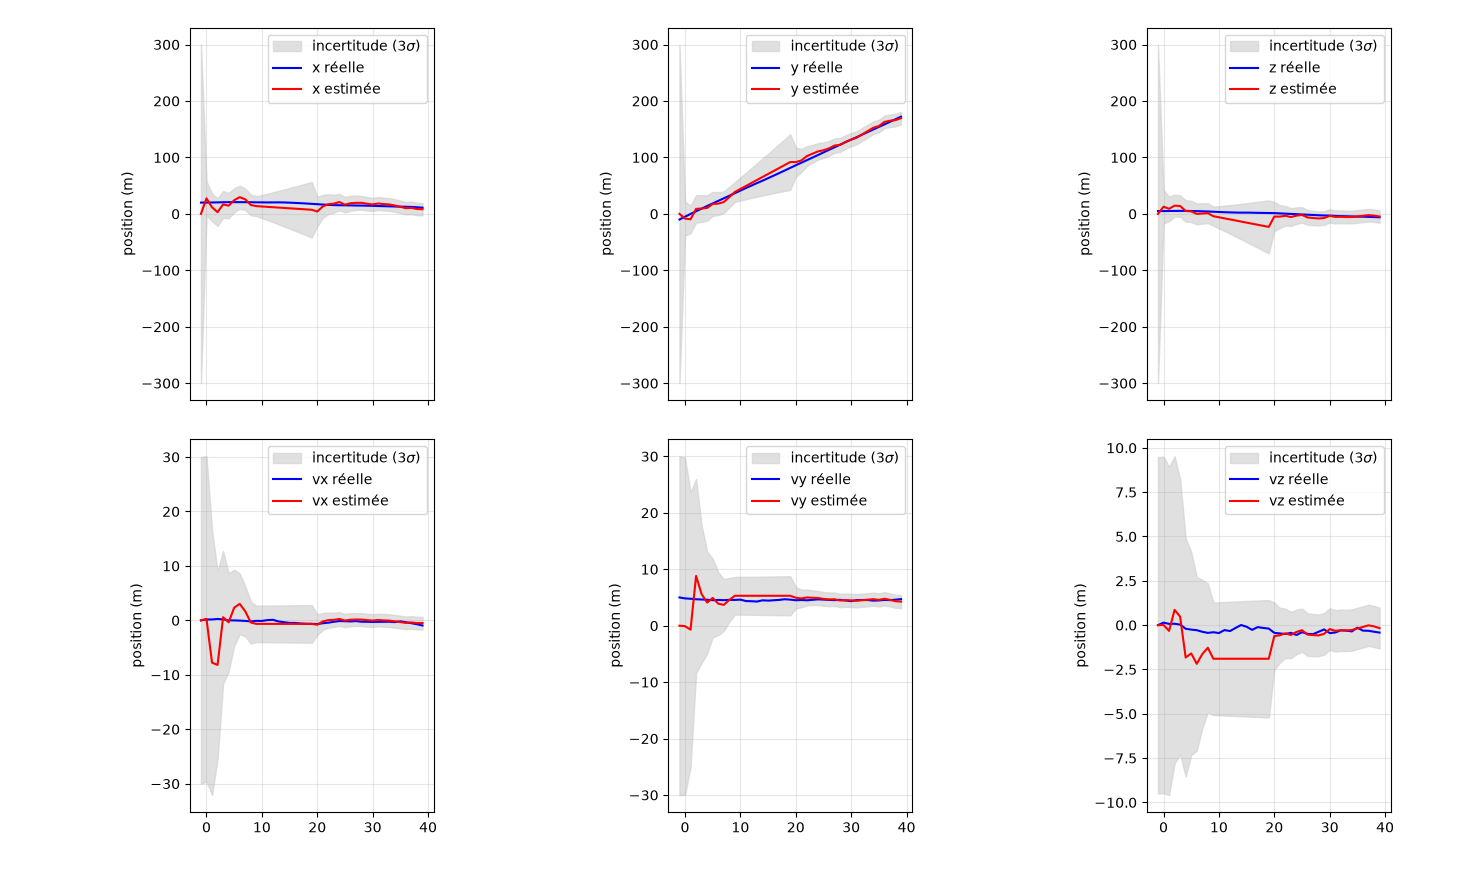
\includegraphics[width=0.8\textwidth]{trou_de_mesure.png}
    \caption{Croissance de l'incertitude pendant le trou de mesure (positions estim\'ees et bandes
    $\pm 3\sigma$).}
    \label{fig:trou}
\end{figure}

\section{Localisation par EKF : odom\'etrie et mod\`eles}\label{sec:q2-systeme}

\subsection{L'odom\'etrie}

L'odom\'etrie (ou navigation \`a l'estime) consiste \`a estimer sa position en int\'egrant ses
d\'eplacements successifs. Le robot conna\^it, par ses encodeurs, le d\'eplacement qu'il pense avoir
effectu\'e \`a chaque pas, exprim\'e dans son rep\`ere local : $u_t = [u_x\ u_y\ u_\theta]^\top$
(avant, lat\'eral, rotation).

La composition de poses (op\'erateur $\oplus$ de SE(2)) d\'efinit le passage de la pose $X$ \`a la
nouvelle pose $X'$ par application du d\'eplacement $U$ :

\begin{equation}
X' = X \oplus U
\quad\Longleftrightarrow\quad
\begin{cases}
\theta' = \theta + u_\theta \\[2pt]
\begin{bmatrix} x' \\ y' \end{bmatrix}
= \begin{bmatrix} x \\ y \end{bmatrix}
+ R(\theta) \begin{bmatrix} u_x \\ u_y \end{bmatrix}
\end{cases}
\label{eq:oplus}
\end{equation}

avec $R(\theta) = \begin{bmatrix} \cos\theta & -\sin\theta \\ \sin\theta & \cos\theta \end{bmatrix}$.
C'est la fonction \texttt{tcomp} du code.

L'odom\'etrie est bruit\'ee : le d\'eplacement r\'eellement mesur\'e est

\begin{equation}
u_t = u_t^{\text{true}} + \eta_t,
\qquad
\eta_t \sim \mathcal{N}(0, Q_{\text{True}}),
\qquad
Q_{\text{True}} = \operatorname{diag}(0.01,\ 0.01,\ 1^\circ)^2 .
\end{equation}

La pose odom\'etrique int\`egre ces d\'eplacements bruit\'es :

\begin{equation}
X^{\text{odom}}_{t+1} = X^{\text{odom}}_t \oplus u_t .
\end{equation}

C'est pourquoi l'odom\'etrie d\'erive : chaque petite erreur s'ajoute \`a la pr\'ec\'edente sans
\^etre corrig\'ee. Sur la figure, la trajectoire odom\'etrique (verte) s'\'ecarte peu \`a peu de la
vraie trajectoire (noire). Le filtre ne conna\^it que la commande bruit\'ee $u_t$, utilis\'ee dans
l'\'etape de pr\'ediction.

\subsection{Mod\`ele d'\'evolution}

La pose pr\'edite \`a partir de la pose courante et du d\'eplacement odom\'etrique :

\begin{equation}
X_{t+1} = f(X_t, U_t) =
\begin{bmatrix}
x_t + x_u \cos\theta_t - y_u \sin\theta_t \\[2pt]
y_t + x_u \sin\theta_t + y_u \cos\theta_t \\[2pt]
\theta_t + \theta_u
\end{bmatrix},
\label{eq:f-model}
\end{equation}

c'est-\`a-dire exactement la composition $X_t \oplus U_t$.

\subsection{Mod\`ele d'observation}

On observe un amer $k$ situ\'e en $(x_k, y_k)$ : la mesure est la distance et la direction de cet
amer, avec un bruit additif $v_t$ :

\begin{equation}
Y_t = h_k(X_t) + v_t =
\begin{bmatrix}
\sqrt{(x_k-x_t)^2 + (y_k-y_t)^2} \\[4pt]
\operatorname{atan2}(y_k-y_t,\ x_k-x_t) - \theta_t
\end{bmatrix} + v_t,
\qquad
v_t \sim \mathcal{N}(0, P_{Y,\text{True}}).
\label{eq:obs-q2}
\end{equation}

o\`u $P_{Y,\text{True}} = \operatorname{diag}(5.0,\ 6^\circ)^2$ est la covariance \emph{r\'eelle} du
bruit de perception (utilis\'ee par le simulateur). Le filtre, lui, utilise la covariance
\emph{suppos\'ee} $P_{Y,\text{Est}} = 10\,P_{Y,\text{True}}$ (voir \eqref{eq:corr-ekf}).

\subsection{Pr\'ediction et correction de l'EKF}

\textbf{Pr\'ediction} (odom\'etrie) :

\begin{equation}
X_{\text{pred}} = f(X_{\text{est}}, u_t),
\qquad
P_{\text{pred}} = A\, P_{\text{est}}\, A^\top + B\, Q_{\text{Est}}\, B^\top,
\end{equation}

o\`u $A = \partial f/\partial X$ et $B = \partial f/\partial U$ sont les jacobiennes du mod\`ele
d'\'evolution.

\textbf{Correction} (perception d'un amer) :

\begin{equation}
\nu = Y_t - h_k(X_{\text{pred}}),
\qquad
S = H\, P_{\text{pred}}\, H^\top + P_{Y,\text{Est}},
\qquad
W = P_{\text{pred}}\, H^\top\, S^{-1},
\label{eq:corr-ekf}
\end{equation}

\begin{equation}
X_{\text{est}} = X_{\text{pred}} + W\,\nu,
\qquad
P_{\text{est}} = P_{\text{pred}} - W\,H\,P_{\text{pred}},
\end{equation}

o\`u $H = \partial h_k/\partial X$ est la jacobienne du mod\`ele d'observation. L'angle $\theta$ et
l'innovation angulaire sont ramen\'es dans $[-\pi, \pi]$ \`a chaque \'etape (fonction
\texttt{angle\_wrap}).

\begin{remark}[Ne pas confondre $P$ et les bruits $Q$, $P_Y$]

\begin{itemize}
\item $P$ (not\'ee \texttt{PEst} / \texttt{PPred} dans le code) est la \textbf{covariance de
l'erreur d'estimation} : l'incertitude que le filtre attribue \`a sa propre estim\'ee
$X_{\text{est}}$. Elle est \emph{calcul\'ee} par le filtre (pr\'ediction puis correction) et ne
provient d'aucun capteur. Il n'existe pas de \emph{vraie} covariance $P$ : c'est une grandeur
interne du filtre, dont la justesse se v\'erifie en la comparant \`a l'erreur r\'eelle
$X_{\text{est}} - X^{\text{true}}$.

\item $Q$ (odom\'etrie) et $P_Y$ (perception) sont les \textbf{covariances de bruit des capteurs}.
Elles existent en deux versions :
\begin{itemize}
\item $Q_{\text{True}}$, $P_{Y,\text{True}}$ : bruit \emph{r\'eel}, utilis\'e par le simulateur pour
produire les donn\'ees bruit\'ees ;
\item $Q_{\text{Est}}$, $P_{Y,\text{Est}}$ : bruit \emph{suppos\'e} par le filtre, utilis\'e dans
\eqref{eq:corr-ekf}. Ici $Q_{\text{Est}} = 10\,Q_{\text{True}}$ et
$P_{Y,\text{Est}} = 10\,P_{Y,\text{True}}$ : le filtre est volontairement pessimiste.
\end{itemize}
\end{itemize}
\end{remark}

\section{Calcul des jacobiennes (Q2)}\label{sec:jacobiennes}

On consid\`ere la localisation par EKF d'un robot dont l'\'etat est
$X = [x\ y\ \theta]^\top$ (position et cap), dont la commande odom\'etrique est
$U = [x_u\ y_u\ \theta_u]^\top$ et qui observe la distance et la direction d'un amer. Trois
jacobiennes interviennent : $A = \partial f/\partial X$, $B = \partial f/\partial U$ et
$H = \partial h/\partial X$.

\subsection{Jacobiennes $A$ et $B$}

\'A partir du mod\`ele d'\'evolution $f(X,U)$ d\'efini pr\'ec\'edemment (voir
\eqref{eq:f-model}), la jacobienne $A = \partial f/\partial X$ vaut

\begin{equation}
A =
\begin{bmatrix}
1 & 0 & -x_u\sin\theta - y_u\cos\theta \\[2pt]
0 & 1 & \phantom{-}x_u\cos\theta - y_u\sin\theta \\[2pt]
0 & 0 & 1
\end{bmatrix},
\label{eq:A}
\end{equation}

et la jacobienne $B = \partial f/\partial U$ est la matrice de rotation $R(\theta)$ compl\'et\'ee
par $1$ sur l'angle :

\begin{equation}
B =
\begin{bmatrix}
\cos\theta & -\sin\theta & 0 \\[2pt]
\sin\theta & \phantom{-}\cos\theta & 0 \\[2pt]
0 & 0 & 1
\end{bmatrix}.
\label{eq:B}
\end{equation}

\subsection{Jacobienne $H$}

\'A partir du mod\`ele d'observation \eqref{eq:obs-q2}, avec $dx = x_k - x$, $dy = y_k - y$ et
$r = \sqrt{dx^2 + dy^2}$ :

La distance donne $\partial r/\partial x = -dx/r$, $\partial r/\partial y = -dy/r$,
$\partial r/\partial\theta = 0$. La direction donne, en rappelant que
$\partial\operatorname{atan2}(y,x)/\partial x = -y/(x^2+y^2)$ et
$\partial\operatorname{atan2}(y,x)/\partial y = x/(x^2+y^2)$ :
$\partial\phi/\partial x = dy/r^2$, $\partial\phi/\partial y = -dx/r^2$,
$\partial\phi/\partial\theta = -1$. D'o\`u

\begin{equation}
H =
\begin{bmatrix}
-\dfrac{dx}{r} & -\dfrac{dy}{r} & 0 \\[8pt]
\phantom{-}\dfrac{dy}{r^2} & -\dfrac{dx}{r^2} & -1
\end{bmatrix}.
\label{eq:H}
\end{equation}

\end{document}
